\documentclass[xcolor=table,aspectratio=169]{beamer}
\usepackage{beamerthemesplit}
\usepackage{wrapfig}
\usetheme{SPbGU}
\usepackage{pdfpages}
\usepackage{amsmath}
\usepackage{cmap} 
\usepackage[T2A]{fontenc} 
\usepackage[utf8]{inputenc}
\usepackage[english,russian]{babel}
\usepackage{indentfirst}
\usepackage{tikz}
\usepackage{multirow}
\usepackage[noend]{algpseudocode}
\usepackage{algorithm}
\usepackage{algorithmicx}
\usetikzlibrary{shapes,arrows}
%usepackage{fancyvrb}
%\usepackage{minted}
%\usepackage{verbments}


\newtheorem{rutheorem}{Теорема}
\newtheorem{ruproof}{Доказательство}
\newtheorem{rudefinition}{Определение}
\newtheorem{rulemma}{Лемма}
\beamertemplatenavigationsymbolsempty

\title[CFPQ]{Теория формальных языков --- это не только написание парсеров}
%\subtitle[YaccConstructor]{Parsing techniques for graph analysis}
% То, что в квадратных скобках, отображается в левом нижнем углу. 
\institute[СПбГУ]{
JetBrains Research, лаборатория языковых инструментов \\
Санкт-Петербургский государственный университет
}

% То, что в квадратных скобках, отображается в левом нижнем углу.
\author[Семён Григорьев]{Семён Григорьев}

\date{17.03.2018}

\definecolor{orange}{RGB}{179,36,31}

\begin{document}
{
\begin{frame}[fragile]
  \begin{tabular}{p{2.5cm} p{9.5cm} p{2cm}}
   \begin{center}
      \includegraphics[height=1.5cm]{pictures/JBLogo3.pdf}
    \end{center}
    &
    \begin{center}
      %\includegraphics[height=1cm]{pictures/logo-2017-transp.png}
      \Huge{ITGM}
    \end{center} 
    &
    \begin{center}
      \includegraphics[height=1.5cm]{pictures/SPbGU_Logo.png}
    \end{center}
  \end{tabular}
  \titlepage
\end{frame}
}

\begin{frame}[fragile]
  \transwipe[direction=90]
  \frametitle{Поиск путей в графах}
  \begin{itemize}
  \item Анализ графов
    \begin{itemize}
        \item Запросы к графовым базам данных
        \item Анализ сетей (социальных, интернет и т.д.)
    \end{itemize}
  \item Статический анализ программ
      \begin{itemize}
        \item Анализ алиасов
        \item Taint analysis
        \item Анализ типов
        \item Статический анализ динамически формируемого кода
      \end{itemize}
   \item ...
  \end{itemize}
\end{frame}

\begin{frame}[fragile]
  \transwipe[direction=90]
  \frametitle{Теория формальных языков}
  \begin{itemize}
  \item Алфавит --- множество символов ($\Sigma, N,$ ...)
  \item Язык --- множество ``слов''
  \item Язык $L$ над алфавитом $\Sigma$: $L(\Sigma) = \{ w | w \in \Sigma^{*} \}$ 
  \item Классы языков
    \begin{itemize}
        \item Регулярные: регулярные выражения (``академические''), конечные автоматы
        \item Контекстно-свободные 
        \item ...
    \end{itemize}
  \item У разных классов разная выразительная сила
    \begin{itemize}
        \item Язык ``правильных'' скобочных последовательностей является контекстно-свободным, но не 
        является регулврным
    \end{itemize}
  \end{itemize}
\end{frame}

\begin{frame}[fragile]
  \transwipe[direction=90]
  \frametitle{Регулярные языки}
  Регулярные языки \\ $\Longleftrightarrow$ регулярные выражения \\ $\Longleftrightarrow$ конечные 
  автоматы \\
  Конечный автомат $M=(\Sigma,Q,P,S,F)$
      \begin{itemize}
        \item $\Sigma$ --- алфавит
        \item $Q$ --- множество состояний
        \item $P \subseteq Q \times \Sigma \times Q$ --- правила перехода из одного состояния в другое
        \item $S \subseteq Q$ --- стартовые состояния
        \item $F \subseteq Q$ --- финальные состояния
    \end{itemize}
\end{frame}

\begin{frame}[fragile]
  \transwipe[direction=90]
  \frametitle{Конечные автоматы}
\begin{center}
        \includegraphics[height=0.4\textheight]{pictures/atm.pdf} 
\end{center}
  \begin{itemize}
  \item $p = v_0 \xrightarrow{l_0} v_1 \xrightarrow{l_1} \cdots v_{n-1}\xrightarrow{l_{n-1}}v_n$ --- путь из стартового состояния в конечное
  \item $w(p) = w(v_0 \xrightarrow{l_0} v_1 \xrightarrow{l_1} \cdots v_{n-1}\xrightarrow{l_{n-1}}v_n) = l_0 l_1 \cdots l_{n-1}$
  \item $L(M) = \{w(p) | p  \text{--- путь из стартового состояния $M$ в конечное}\}$
  \item $L(M) = \{aaa; bb; aaabb; aaabbaaabbbb, \dots\}$
  \end{itemize}

\end{frame}


\begin{frame}[fragile]
  \transwipe[direction=90]
  \frametitle{Контекстно-свободные языки}
Контекстно-свободная грамматика $\mathbb{G}=(\Sigma,N,P,S)$ 
  \begin{itemize}
      \item $\Sigma$ --- терминальный алфавит
      \item $N$ --- нетерминальный алфавит
      \item $P$ --- правила вывода
      \item $S \in N$ --- стартовый нетерминал
  \end{itemize}

Контекстно свободная граммтика для языка $L=\{a^n b^n; n \geq 1\}$ с явным выделением ``середины'' \\
\begin{center}
   \[
\begin{array}{rl} 
   0:& S \rightarrow a \ S \ b \\
   1:& S \rightarrow Middle \\
   2:& Middle \rightarrow a \ b
\end{array}
\]
\end{center}

Грамматика как правила переписывания:
 
    \begin{itemize}
        \item $S \xrightarrow{1} Middle \xrightarrow{2} ab$
        \item $S \xrightarrow{0} a\ S\ b \xrightarrow{0} aa\ S\ bb \xrightarrow{1} aa\ Middle\ bb \xrightarrow{2} aaabbb$
    \end{itemize}

\end{frame}

\begin{frame}[fragile]
  \transwipe[direction=90]
  \frametitle{Поиск путей с контекстно-свободными ограничениями}
  \begin{itemize}
  \item $\mathbb{G} = (\Sigma, N, P)$ --- контекстно-свободная грамматика
  \item $G = (V,E,L)$ --- ориентированный граф, $E \subseteq V\times L \times V$, $L\subseteq \Sigma$
  \item $p = v_0 \xrightarrow{l_0} v_1 \xrightarrow{l_1} \cdots v_{n-1}\xrightarrow{l_{n-1}}v_n$ --- путь в графе $G$
  \item $w(p) = w(v_0 \xrightarrow{l_0} v_1 \xrightarrow{l_1} \cdots v_{n-1}\xrightarrow{l_{n-1}}v_n) = l_0 l_1 \cdots l_{n-1}$
  \item $R =\{ p \ | \ \exists N_i \in N (w(p) \in L(\mathbb{G},N_i))\}$
  \begin{itemize}
    \item Стартовый нетерминал можно зафиксировать заранее
    \item \textbf{Проблема:} множество $R$ может быть бесконечным
  \end{itemize}
  \end{itemize}
\end{frame}

\begin{frame}[fragile]
  \transwipe[direction=90]
  \frametitle{Пример}
%\begin{figure}[ht]
Входной граф 
\vspace{-0.5cm}
\begin{center}
        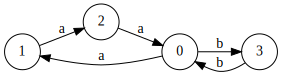
\includegraphics[height=0.2\textheight]{pictures/input.pdf} 
\end{center}
Запрос --- грамматика $G$ для языка $L=\{a^n b^n; n \geq 1\}$ с явным выделением середины пути \\
\begin{center}
   \[
\begin{array}{rl} 
   0:& S \rightarrow a \ S \ b \\
   1:& S \rightarrow Middle \\
   2:& Middle \rightarrow a \ b
\end{array}
\]
\end{center}
\vspace{0.8em}
Ответ --- бесконечное множество путей
\begin{itemize}
\item $p_1 = 0\xrightarrow{a}1\xrightarrow{a}2\xrightarrow{a}0\xrightarrow{b}3\xrightarrow{b}0\xrightarrow{b}3$
\item $p_2 = 0\xrightarrow{a}1\xrightarrow{a}2\xrightarrow{a}0\xrightarrow{a}1\xrightarrow{a}2\xrightarrow{a}0\xrightarrow{b}3\xrightarrow{b}0\xrightarrow{b}3\xrightarrow{b}0\xrightarrow{b}3\xrightarrow{b}0$
\item ...
\end{itemize}

\end{frame}

\begin{frame}[fragile]
  \transwipe[direction=90]
  \frametitle{Структурное представление результата запроса}
\vspace{-0.3cm}
\begin{figure}[ht]
    \centering
        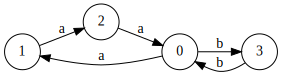
\includegraphics[width=0.45\textwidth]{pictures/input.pdf} \\
        Входной граф
\end{figure}
\vspace{-0.2cm}
\begin{center}
\begin{tabular}{  c  c  c  }
      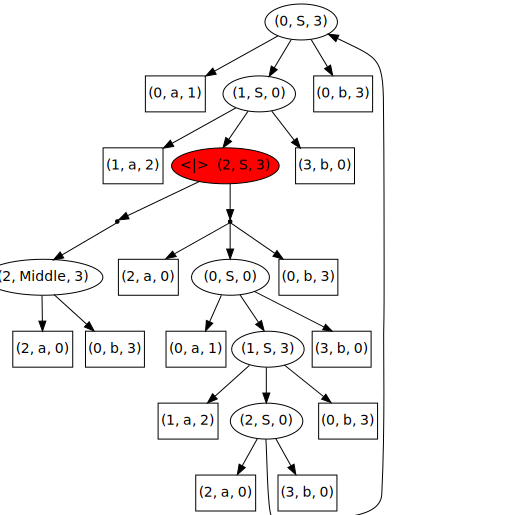
\includegraphics[height=4.5cm]{pictures/AnBn.pdf}
    &
      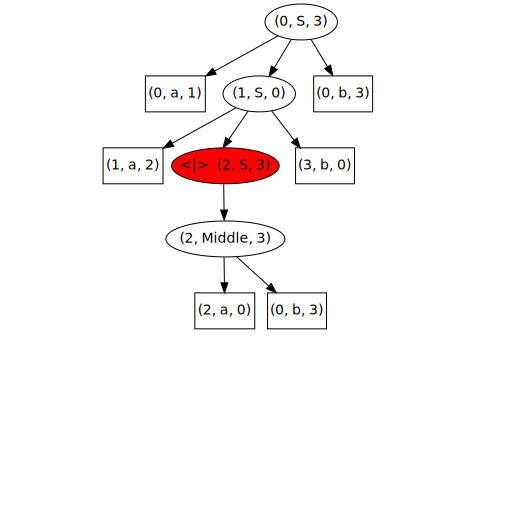
\includegraphics[height=4.5cm]{pictures/AnBn_2.pdf}
    &
      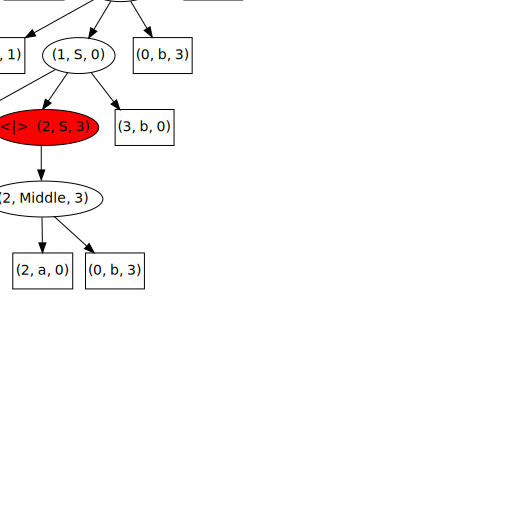
\includegraphics[height=4.5cm]{pictures/AnBn_1.pdf}

\\
\small{Результат (SPPF)}
& \small{Дерево вывода пути $p_1$}
& \small{Дерево вывода пути $p_2$}
  \end{tabular}
\end{center}                
\end{frame}

\begin{frame}[fragile]
  \transwipe[direction=90]
  \frametitle{Пример: извлечение путей}
\begin{center}

\begin{minipage}{0.4\textwidth}
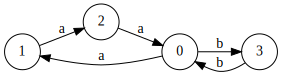
\includegraphics[width=0.9\textwidth]{pictures/input.pdf}
\\
Путь: $0\xrightarrow{a}1\xrightarrow{a}2\xrightarrow{a}0\xrightarrow{b}3\xrightarrow{b}0\xrightarrow{b}3$
\end{minipage}
~
\begin{minipage} {0.57\textwidth}
\includegraphics[width=0.99\textwidth]{pictures/AnBn_2_m.pdf}
\end{minipage}

        
\end{center}                
\end{frame}


\begin{frame}[fragile]
  \transwipe[direction=90]
  \frametitle{Почему это работает}
Замкнутость КС языков относительно пересечения с регуляными
\pause
\vspace{-0.2cm}
\begin{center}
\begin{tabular}{  l p{4cm} l  }
    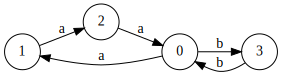
\includegraphics[width=0.35\textwidth]{pictures/input.pdf}
    & &
$
 
\begin{array}{rl} 
   0:& S \rightarrow a \ S \ b \\
   1:& S \rightarrow Middle \\
   2:& Middle \rightarrow a \ b
\end{array}

$
\end{tabular}

\vspace{-0.65cm}
\pause

\begin{tabular}{  l p{2cm}  l  }
    \raisebox{-0.5\totalheight}{\includegraphics[width=0.29\textwidth]{pictures/AnBn_m.pdf}}
    &
    &
$
\begin{array}{rl} 
   (0,S,3) & \rightarrow (0,a,1) \ (1,S,0) \ (0,b,3) \\
   (1,S,0) & \rightarrow (1,a,2) \ (2,S,3) \ (3,b,0) \\
   (2,S,3) & \rightarrow (2,a,0) \ (0,S,0) \ (0,b,3) \\
   (2,S,3) & \rightarrow (2,Middle,3)                \\
   (0,S,0) & \rightarrow (0,a,1) \ (1,S,3) \ (3,b,0) \\
   (1,S,3) & \rightarrow (1,a,2) \ (2,S,0) \ (0,b,3) \\
   (2,S,0) & \rightarrow (2,a,0) \ (0,S,3) \ (3,b,0) \\
   (0,Middle,3) & \rightarrow (2,a,0) \ (0,b,3)  \\
\end{array}
$

\end{tabular}
\end{center}                
\end{frame}


\begin{frame}[fragile]
  \transwipe[direction=90]
  \frametitle{Примеры применения}
  \begin{itemize}
  \item Графовые базы данных и семантические сети
    \begin{itemize}
        \item Same-generation query (и модификации), similarity query (и модификации)
        \item \emph{Sevon P., Eronen L.} ``Subgraph queries by context-free grammars.'' 2008
        \item \emph{Zhang X. et al.} ``Context-free path queries on RDF graphs.'' 2016
        \item \emph{Hellings J.} ``Conjunctive context-free path queries.'' 2014
    \end{itemize}
    \item Статический анализ кода
    \begin{itemize}
        \item \emph{Thomas Reps et al.} ``Precise interprocedural dataflow analysis via graph reachability.'' 1995 
        \item \emph{Qirun Zhang et al.}  ``Efficient subcubic alias analysis for C.'' 2014
        \item \emph{Dacong Yan et al.} ``Demand-driven context-sensitive alias analysis for Java.'' 2011
        \item \emph{Jakob Rehof and Manuel Fahndrich.} ``Type-base flow analysis: from polymorphic subtyping to CFL-reachability.'' 2001
    \end{itemize}

  \end{itemize}

\end{frame}


\begin{frame}[fragile]
  \transwipe[direction=90]
  \frametitle{Факты}
  \begin{itemize}
  \item В данной области существуют открытые проблемы
    \begin{itemize}
        \item Например, существует ли алгоритм со сложностью $O(|V|^{3-\varepsilon}), \varepsilon > 0$
    \end{itemize}
  \item В данной области применимы решения из ``классического'' синтаксического анализа
    \begin{itemize}
        \item Алгоритмы: CYK, (Generalized) LL, (Generalized) LR, Эрли, ...
        \item Техники: комбинаторы, генераторы парсеров, ... 
        \item Оптимизации: использование GPGPU, специальные структуры данных (сжатое представление леса разбора, структурированный в виде графа стек), ...
    \end{itemize}
  \item Из-за существенно бОльших объёмов данных требуются специальные оптимизации (распределённые вычисления, параллельные вычисления, ...)
  \end{itemize}

\end{frame}

\begin{frame}[fragile]
  \transwipe[direction=90]
  \frametitle{Обобщённый LL для выполнения КС запросов к графам}

\begin{itemize} 
\item Основа --- обобщённый LL (Generalized GLL, GLL)
\begin{itemize} 
  \item \emph{Scott E., Johnstone A.} ``GLL parsing''
\end{itemize}
\item Поддерживает произвольные контекстно-свободные граммтики (неоднозначные, леворекурсивные)
\item Строит сжатое представление леса разбора (Sharep Packed Parse Forest, SPPF) --- конечное представление бесконечного ответа
\item \emph{Semyon Grigorev and Anastasiya Ragozina.} ``Context-free path querying with structural representation of result.'' 2017
\item Реализован на F\#: \url{https://github.com/YaccConstructor/YaccConstructor}
\end{itemize}
\end{frame}


\begin{frame}
  \transwipe[direction=90]
  \frametitle{Свойства алгоритма}

Пусть на входе граф $M=(V,E,L)$, тогда
\begin{itemize} 
\item Пространственная сложность предложенного алгоритма $O(|V|^3 + |E|)$
\item Временная сложность предложенного алгоритма $O\left(|V|^3*\max\limits_{v \in V}\left(deg^+\left(v\right)\right)\right)$
\item Результирующий SPPF имеет размер $O(|V'|^3 + |E'|)$, где $M'=(V',E',L')$ --- подграф $M$, содержащий только искомые пути
\end{itemize}

\end{frame}

\begin{frame}[fragile]
\transwipe[direction=90]
\frametitle{Экспериментальное исследование: запросы}
%\centering
\begin{figure}[ht]
%   \begin{center}
   \centering
%   \begin{subfigure}[b]{0.4\textwidth}

   \[
\begin{array}{rl}
   0: & \textbf{S} \rightarrow \text{\textit{subClassOf}}^{-1} \ \textbf{S} \ \text{\textit{subClassOf}} \\ 
   1: & \textbf{S} \rightarrow \text{\textit{type}}^{-1} \ \textbf{S} \ \text{\textit{type}} \\ 
   2: & \textbf{S} \rightarrow \text{\textit{subClassOf}}^{-1} \ \text{\textit{subClassOf}} \\ 
   3: & \textbf{S} \rightarrow \text{\textit{type}}^{-1} \ \text{\textit{type}} \\ 
\end{array}
\]
   Грамматика для запроса Query 1
   \end{figure}
\begin{figure}[h]%{0.4\textwidth}
   \centering

   \[
\begin{array}{rl}
   0: & \textbf{S} \rightarrow \textbf{B} \ \text{\textit{subClassOf}} \\ 
   1: & \textbf{S} \rightarrow \text{\textit{subClassOf}} \\ 
   2: & \textbf{B} \rightarrow \text{\textit{subClassOf}}^{-1} \ \textbf{B} \ \text{\textit{subClassOf}} \\
   3: & \textbf{B} \rightarrow \text{\textit{subClassOf}}^{-1} \ \text{\textit{subClassOf}} \\ 
\end{array}
\]
   Грамматика для запроса Query 2

   \end{figure}

\end{frame}


\begin{frame}[fragile]
\transwipe[direction=90]
\frametitle{Экспериментальное исследование: результаты}
\centering
\rowcolors{1}{}{lightgray}
\begin{tabular}{  c | c | c | c | c | c | c }
%\hline
Ontology & \#edg & \multicolumn{3}{c|}{Query 1} & \multicolumn{2}{c}{Query 2} \\
\cline{3-7}
& & CYK\footnote{Zhang, et al. ``Context-free path queries on RDF graphs.''} (ms) & GLL (ms) & \#result & GLL (ms) & \#result \\
\hline 
\hline
skos        & 252  & 1044  & 10 & 810 & 1 & 1 \\
generations & 273  & 6091  & 19 & 2164 & 1 & 0 \\
travel      & 277  & 13971 & 24 & 2499 & 1 & 63 \\
univ-bench  & 293  & 20981 & 25 & 2540 & 11 & 81 \\
people-pets & 640  & 82081 & 89 & 9472 & 3 & 37 \\
atom-primitive & 425 & 515285 & 255 & 15454 & 66 & 122 \\
\shortstack{biomedical- \\ measure-primitive} & 459 & 420604 & 261 & 15156 & 45 & 2871 \\
pizza       & 1980 & 3233587 & 697 & 56195 & 29 & 1262 \\
wine        & 1839 & 4075319 & 819 & 66572 & 8 & 133 \\
%\hline
\end{tabular}

\end{frame}

\begin{frame}[fragile]
  \transwipe[direction=90]
  \frametitle{Использование GPGPU для выполнения КС запросов к графам}

\begin{itemize} 
\item Отправная точка --- синтаксический анализ линейного входа через перемножение матриц
\begin{itemize}     
  \item \emph{Valiant L.} ``General context-free recognition in less than cubic time.'' 1974
\end{itemize}
\item Основан на матричных опреациях --- позволяет использовать GPGPU
\begin{itemize}     
  \item Можно использовать разреженное представление и готовые библиотеки для работы с ним
\end{itemize}
\item Применим для других классов грамматик (например, конъюнктивных)
\item \emph{Rustam Azimov, Semyon Grigorev.} ``Context-Free Path Querying by Matrix Multiplication.'' 2017
\item Реализован на F\#: \url{https://github.com/YaccConstructor/YaccConstructor}
\end{itemize}
\end{frame}


\begin{frame}
  \transwipe[direction=90]
  \frametitle{Свойства алгоритма}

Пусть на входе граф $M=(V,E,L)$ и грамматика $\mathbb{G} = (N, \Sigma, P)$, тогда
\begin{itemize} 
\item Пространственная сложность предложенного алгоритма $O(|N||V|^2)$
\item Временная сложность предложенного алгоритма $O(|V|^2 |N|^3(BMM(|V|) + BMU (|V|)))$
\begin{itemize} 
\item $BMM(n)$ --- время, необходимое для умножения сложения булевых матриц $n\times n$
\item $BMU(n)$ --- время, необходимое для поэлементного сложения булевых матриц $n\times n$
\end{itemize}

\end{itemize}

\end{frame}


\begin{frame}[fragile]
\transwipe[direction=90]
\frametitle{Экспериментальное исследование: результаты}
\centering
\rowcolors{1}{}{lightgray}
\begin{tabular}{  c | c | c | c | c | c }
%\hline
Ontology & \#edg & \multicolumn{2}{c|}{Query 1} & \multicolumn{2}{c}{Query 2} \\
\cline{3-6}
& & GLL (ms) & GPGPU (ms)  & GLL (ms) & GPGPU (ms) \\
\hline 
\hline
skos        & 252    & 10   & 12  & 1   & 1 \\
generations & 273    & 19   & 13  & 1   & 0 \\
travel      & 277    & 24   & 30  & 1   & 10 \\
univ-bench  & 293    & 25   & 15  & 11  & 9 \\
people-pets & 640    & 89   & 32  & 3   & 6 \\
atom-primitive 
            & 425    & 255  & 22  & 66  & 2 \\
\shortstack{biomedical- \\ measure-primitive} 
            & 459    & 261  & 20  & 45  & 24 \\
pizza       & 1980   & 697  & 24  & 29  & 23 \\
wine        & 1839   & 819  & 54  & 8   & 6 \\
$g_{1}$     & 11840  & 1926 & 82  & 167 & 38\\
$g_{2}$     & 19600  & 6246 & 185 & 46  & 21\\
$g_{3}$     & 20832  & 7014 & 127 & 393 & 40\\

%\hline
\end{tabular}

\end{frame}

\begin{frame}
  \transwipe[direction=90]
  \frametitle{Направления}

\begin{itemize} 
\item Разработка эффективных ``практичных'' алгоритмов и реализация библиотек
\begin{itemize} 
\item Интеграция с существующими языками запросов к графам
\item Интеграция с существующими интефейсами к граф-структурированным данным
\end{itemize}

\item Формулировка прикладных задач в терминах КС запросов к графам
\begin{itemize} 
\item Сравнение с ``классическими'' решениями
\end{itemize}

\end{itemize}

\end{frame}

            
\begin{frame}
\transwipe[direction=90]
\frametitle{Контакты}
\begin{itemize}
  \item Почта: \url{semen.grigorev@jetbrains.com}
  \item GitHub-сообщество YaccConstructor: \url{https://github.com/YaccConstructor}
\end{itemize}
\end{frame}
\end{document}
